\documentclass[11pt]{scrartcl}
\usepackage{graphicx}
\usepackage{float}
\usepackage{amsmath}
 
\begin{document}
\title{Praktiukumsarbeit zum Praktikum Regelungstechnik}
\author{Christian Küllmer, Jonas Kallweidt, Leon Blum}
\date{\today{}, Kassel}
\maketitle
\newpage
%Inhaltsverzeichnis
\renewcommand{\contentsname}{Inhaltsverzeichnis}
\tableofcontents
\newpage

%Mathlab Aufgabe
\section{Rechnerteil Aufgaben aus Kapitel 9.3. des Praktikumsskrips}
In diesem Anteil geht es um die in Aufgabe 9.3a. Dieser bezeichnet das Aufstellen der Gleichungen aus den gegeben Gleichungen. Die Gleichungen sind gegen als Blockschaltbild gegeben. Diese werden jetzt übersetzt in Mathlab Simulink.

\begin{itemize}
\item Startwerte
Als Startwerte wurde gegeben:

\begin{align}
   	m &= 7\, kg
\end{align}
\begin{align}
   	l &= 1\, m
\end{align}
\begin{align}
   	g &= 9,81\, \frac{m}{s^2}
\end{align}
\begin{align}
   	c &= 1
\end{align}

	
	


\item Gegebenes Blockschaltbild:
\begin{figure}[H]
	\centering
	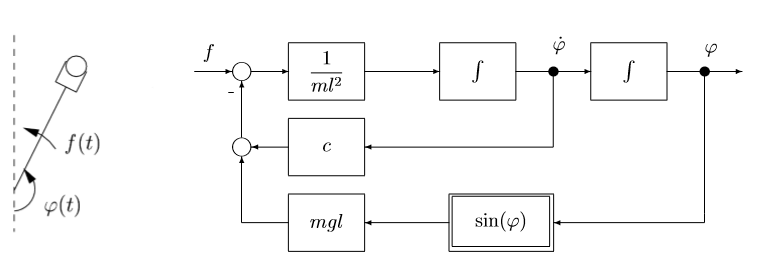
\includegraphics[width=0.6\textwidth]{Aufgabe9aMotorarm.png}
	\caption{Motorarmmodell als Blockschaltbild}
	\label{img:grafik-dummy}
\end{figure}
\begin{figure}[H]
	\centering
	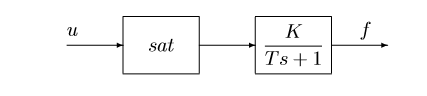
\includegraphics[width=0.6\textwidth]{Aufgabe9aStreckeMotor.png}
	\caption{Modell des Motors als Blockschaltbild}
	\label{img:grafik-dummy}
\end{figure}
\item Gebautes Simulink Modell:
\begin{figure}[H]
	\centering
	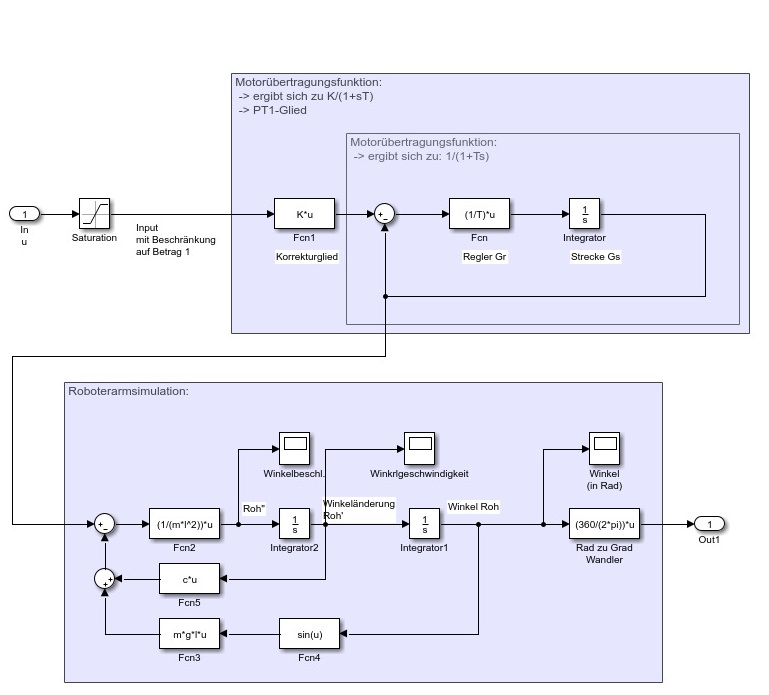
\includegraphics[width=0.7\textwidth]{SimulinkModell.jpeg}
	\caption{in Simulink gebautes Modell des Systems des Roboterarms}
	\label{img:grafik-dummy}
\end{figure}
\end{itemize}

%Aufgabe a
\subsection{Aufgabe a)}



\subsection{Aufgabe b)}

\subsection{Aufgabe c)}

%Präsensversuche
\section{Versuch Antrieb}

\section{Versuch Schwebekörper}

\section{Versuch Kran}

%Modell zum Einfügen eines Bildes
%\begin{figure}[H]
%	\centering
%	\includegraphics[width=0.8\textwidth]{}
%	\caption{Teamlogo: Team A}
%	\label{img:grafik-dummy}
%\end{figure}
Hallo
\end{document}